\DiaryEntry{Chi-Square Distribution}{2016-01-18}{Stochastic}

If \(Z_1, \ldots, Z_k\) are iid standard normal RVs, then the sum of
their squares,

\[
Q_k = \sum_{i=1}^k Z_i^2
\]

is distributed according to the chi-squared distribution with \(k\)
degrees of freedom, denoted as \(Q \sim \chi^2 (k)\).

The pdf of a chi-squared distribution with \(k\) degrees of freedom has the following form

\[
f(x; k) = \frac{ x^{k/2-1} e^{-x/2} }{ 2^{k/2} \Gamma(\frac{k}{2}) }; \, x \geq 0
\]

A plot of the distribution for different values of \(k\) can be seen
below:

\begin{figure}[H]
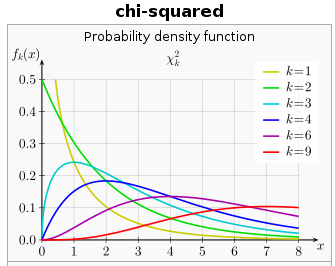
\includegraphics{images/chi-square_01.png}
\end{figure}

For increasing \(k\), the peak of the distribution moves to the right as more and more terms are involved in the summation. This is also consistent with the mean of the chi-squared distribution being equal to \(k\).

\subsubsection{Limit values for \(x=0\)}

For \(k=1\), we have:

\begin{equation}
\label{keqone}
f(x;1) = \frac{e^{-x/2}}{\sqrt{2\pi}\sqrt{x}}
\end{equation}

and this becomes infinity for \(x \rightarrow 0\).

For \(k=2\), we obtain

\[
f(x;2) = \frac{1}{2} e^{-x/2}
\]

and this becomes \(1/2\) for \(x \rightarrow 0\).

Finally, for \(k \geq 3\), the x moves into the numerator, thereby
causing the pdf to become zero for \(x \rightarrow 0\).

\subsubsection{Open Question}

The pdf at \(x=0\) equals the probability that \(Q=0\); i.e.

\[
P\left\{\sum_{i=1}^k Z_i^2=0\right\}
\]

It would be interesting to understand, why this probability is non-zero for 1 and 2 normal RVs and only becomes zero for 3 or more RVs.

Actually, the difference has a smaller effect on the cdf. Here, the
value \(f(0;k)\) only affects the slope of the cdf \(F_Q(x)\) at
\(x=0\). Therefore, the cdf has a zero slope at \(x=0\) for
\(k \geq 3\).

\subsubsection{Special Case \(k=1\)}

In this case, we have \(Q_1 = Z_1^2\) which is actually a RV transformation. We can directly use results from the next entry and arrive at

\[
f(x;1) = \frac{1}{\sqrt{x}} f_Z(\sqrt{x}) = \frac{1}{\sqrt{2 \pi x}} e^{- (\sqrt{x})^2 / 2 } = \frac{1}{\sqrt{2 \pi x}} e^{- x / 2 }
\]

which is exactly the result from \eqref{keqone}.
